\documentclass[12pt, a4paper]{article}
\usepackage[utf8]{inputenc}
\usepackage{hyperref}
\usepackage[left=1.00in, right=1.00in, top=1.00in, bottom=1.00in]{geometry}
\usepackage{graphicx}
\graphicspath{ {./} }
\title{CS348 Project Milestone 1}
\author{Abdullah Bin Assad\and Chandana Sathish \and Lukman Mohamed \and Vikram Subramanian \and Dhvani Patel}
\begin{document}
\maketitle

\section*{Application description}
\subsection*{Application User}
We are creating an interactive web app for people interested in exploring crime data in the Greater Toronto Area. People who wish to assess how safe a neighbourhood is before investing in a new property or novice drivers trying to avoid accident-prone roads or just people curious about crime rates around them can greatly benefit from our application.
\subsection*{Interaction with the app}
A user would simply search for a query (as seen on the demo application) using the drop-down on certain words in the question to tailor the search to their needs. For example, “I want to explore bicycle theft crimes in 2019 (year) citywide on a bar chart” can be one of the many queries a user selects. Alternatively, a user can also pick from a list of predefined queries (not in the demo yet) if they are unsure about where to start. Once the user clicks “OK”, the page updates to display the requested query and allows them to change the representation/visualization of the data as well as further refine their search with more options. We also plan on adding additional features as follows.
\subsection*{Key features}
\begin{enumerate}
\item Filter crime/traffic events (starter question with drop-down for filtering different columns as seen in demo) and show results on a table
\item Display crime data
\begin{itemize}
\item bar chart, line chart, and pie chart
\item map, heat map
\end{itemize}
\item Create predefined complex queries in the form of question and answer
\begin{itemize}
    \item Example - Where should I park by bike in this neighbourhood, where should I drive as a new driver, is there a correlation between education/demographic and crime?
\end{itemize}
\item Provide users with information on closest police division or which neighborhood they are situated in based on the address they provide us with
\item Report a crime
\item Interactive “How well do you know your city” feature
\begin{itemize}
    \item Let the user guess certain values from a query they select, then show them the actual results and tell them how close they were
    \item Store user guess average and tell them how they compare against other users who tried guessing the same value
\end{itemize}
\end{enumerate}
\subsection*{Data}
The tables we get from the Toronto Police Open Data ( \url{https://data.torontopolice.on.ca/pages/open-data}) are a little difficult to work with. Therefore, we create a data parser (in code.zip) to convert it to .csv files that fulfill our requirements. Sample data is part of the code.zip as csv files (ex. Neighbourhood.csv, CrimeEvent.csv).
\subsection*{System support}
Our interface will consist of an interactive web-app. We will be using Azure to host our database and run a MySQL instance. This setup is ideal and efficient for building a web app such as ours. Azure and MySQL are modern, scalable, efficient and flexible. We will be using Node.js with an Express.js server as our back-end to interact with the database. For the front-end, we will be using the React library. Thus, our web application code mostly consists of JavaScript. Members of our group have experience with Node.js and React which gives us an excellent basis for our project.

\section*{Design database schema}
\subsection*{List of assumptions}
\begin{itemize}
    \item all reported times of incidents are either in or after 2014
    \item for regular crimes and traffic accidents, the time and place of the incident are recorded accurately and not left out (not NULL mostly)
    \item the level and standard of reporting crimes is consistent in all neighbourhoods (required for useful analysis and comparison among neighbourhoods)
    \item the cause of the traffic accident is taken from testimonies of all parties involved and is not one sided (although hard to avoid survivorship bias)
    \item the police arrive at the scene of an accident within reasonable time to be able to assess the road conditions leading up to the cause of the accident
    \item all parties involved in an accident are accounted for (driver, passengers, pedestrians)
    \item the status of stolen bikes is updated as best as possible (most bikes are never recovered)
\end{itemize}
\subsection*{E/R diagram}
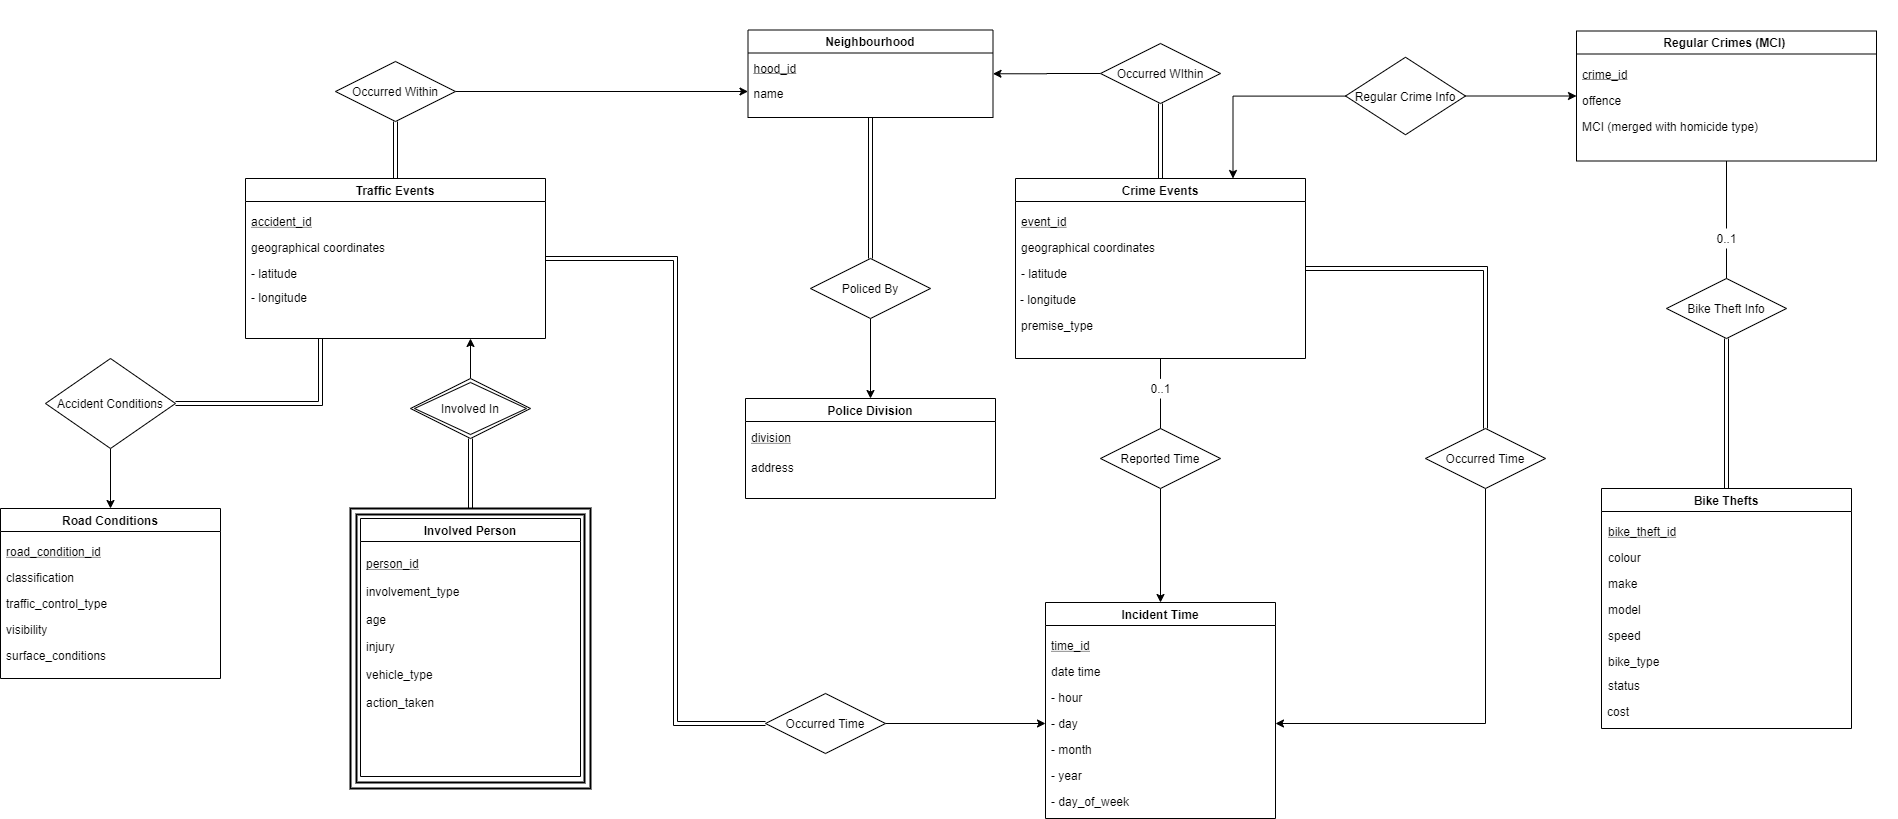
\includegraphics[scale=0.25]{ER Diagram.png}
Note: Check the standalone image of the ER diagram if this one is too small.
\subsection*{Relational Data Model}
\begin{itemize}
    \item IncidentTime
    \begin{itemize}
        \item \underline{time\_id}
        \item hour
        \item day
        \item month
        \item year 
        \item day\_of\_week
    \end{itemize}
    \item PoliceDivision
        \begin{itemize}
        \item \underline{division}
        \item address
    \end{itemize}
    \item Neighbourhood
        \begin{itemize}
        \item \underline{hood\_id}
        \item name
        \item division (Foreign Key Referencing PoliceDivision(division))
    \end{itemize}
    \item BikeTheft
        \begin{itemize}
        \item \underline{bike\_theft\_id}
        \item colour
        \item make
        \item model
        \item speed
        \item bike\_type
        \item status
        \item cost
    \end{itemize}
    \item RegularCrime
        \begin{itemize}
        \item \underline{crime\_id}
        \item offence
        \item MCI
    \end{itemize}
    \item CrimeEvent
        \begin{itemize}
        \item \underline{event\_id}
        \item occurrence\_time\_id (Foreign Key Referencing IncidentTime(time\_id))
        \item reported\_time\_id (Foreign Key Referencing IncidentTime(time\_id))
        \item crime\_id (Foreign Key Referencing RegularCrime(crime\_id))
        \item bike\_theft\_id (Foreign Key Referencing BikeTheft(bike\_theft\_id))
        \item hood\_id (Foreign Key Referencing Neighbourhood(hood\_id))
        \item latitude
        \item longitude
        \item premise\_type
    \end{itemize}
    \item InvolvedPerson
    \begin{itemize}
        \item \underline{accident\_id} (Foreign Key Referencing TrafficEvent(accident\_id))
        \item \underline{person\_id}
        \item involvement\_type,
        \item age
        \item injury
        \item vehicle\_type
        \item action\_taken
    \end{itemize}
    \item RoadCondition
    \begin{itemize}
        \item \underline{road\_condition\_id}
        \item classification
        \item traffic\_control\_type
        \item visibility
        \item surface\_condition
    \end{itemize}
    \item TrafficEvent
    \begin{itemize}
        \item \underline{accident\_id}
        \item occurrence\_time\_id (Foreign Key Referencing IncidentTime(time\_id))
        \item road\_condition\_id (Foreign Key Referencing RoadCondition(road\_condition\_id))
        \item hood\_id (Foreign Key Referencing Neighbourhood(hood\_id))
        \item latitude
        \item longitude
    \end{itemize}
\end{itemize}
\end{document}